% how to assemble Vidar III, as it stood at irec 2017

%%%%%%%%%%%%%%%%%%%%%%%%%%%%%%%%%%%%%%%%%%%%%%%%%%%%%%%%%%%%%%%%%%%%%%%%%%%%%%%%%
% Waterloo Rocketry Standard template for operations procedures                 %
% Copyright claimed by Aaron Morrison (akmorris@uwaterloo.ca)                   %
% Any commercial entity wishing to use this template in any way must provide    %
% to Waterloo Rocketry, one two-four (24 pack) of a non-shitty                  %
% type of beer or an amount of Canadian dollars roughly equalling               %
% the current cost of such a purchase. If you do so, then use it                %
% however you want, and I claim in no way that it compiles properly,            %
% and I take no responsibilty for any loss you incurr from using                %
% this template, and make no promises to support you in any technical           %
% capacity for sustained use.                                                   %
%%%%%%%%%%%%%%%%%%%%%%%%%%%%%%%%%%%%%%%%%%%%%%%%%%%%%%%%%%%%%%%%%%%%%%%%%%%%%%%%%
\documentclass[letter]{article}

%% margins and fonts
\usepackage[margin=1in]{geometry}
\renewcommand{\familydefault}{\sfdefault}

% begin package imports -- {{{
\usepackage{amsmath}
\usepackage{graphicx}
\usepackage[dvipsnames]{xcolor}
\usepackage{tabto}
\usepackage{titling}
\usepackage[iso,german]{isodate}
% end package imports -- }}}

% begin set section title styles -- {{{
\usepackage{titlesec}
\titleformat{\section} {\setcounter{checklistnum}{0} \normalfont\Large\bfseries}{}{0em}{}[{\titlerule[0.8pt]}]
\titleformat{\subsection} {\setcounter{checklistnum}{0} \normalfont\large}{}{0em}{}[{\titlerule[0.6pt]}]
% end set section title styles -- }}}

% begin checklist symbols definition -- {{{
\usepackage{enumitem,amssymb}
\newcounter{checklistnum}
\setcounter{checklistnum}{0}
\DeclareRobustCommand{\checklistnumber}{\refstepcounter{checklistnum}\thechecklistnum}
\newlist{checklist}{itemize}{6}
\setlist[checklist,1]{
label={\color{gray}\checklistnumber}\hspace{2em}$\square$,
leftmargin=0em,
itemindent=2em
}
\setlist[checklist,2]{
label={\color{gray}\checklistnumber}\hspace{4em}$\square$,
leftmargin=0em,
itemindent=4em
}
\setlist[checklist,3]{
label={\color{gray}\checklistnumber}\hspace{6em}$\square$,
leftmargin=0em,
itemindent=6em
}
\setlist[checklist,4]{
label={\color{gray}\checklistnumber}\hspace{8em}$\square$,
leftmargin=0em,
itemindent=8em
}
\setlist[checklist,5]{
label={\color{gray}\checklistnumber}\hspace{10em}$\square$,
leftmargin=0em,
itemindent=10em
}
\setlist[checklist,6]{
label={\color{gray}\checklistnumber}\hspace{12em}$\square$,
leftmargin=0em,
itemindent=12em
}
% end checklist symbols definition -- }}}

% begin personnel macro -- {{{
\newcommand{\operator}[4]{%
  \expandafter\newcommand\csname #1\endcsname{{\color{#2}\textbf{#3}}\phantom{}}
  \expandafter\newcommand\csname #1full\endcsname{{\color{#2}\textbf{#4 [#3]}}\phantom{}}
}
% end personnel macro -- }}}

\pagenumbering{gobble}

\usepackage{gensymb}
\usepackage{hyperref}

\title{
\Huge Rocket Assembly Procedure\\
\vspace{1cm}
\Large Vidar III, IREC 2017}

\begin{document}

% begin titlepage -- {{{
\begin{center}
\vspace*{7cm}
\hspace{7em}
\includegraphics[width=30em]{common/mono_horizontal_standard}
\newline
\rule{50em}{2pt}

\vspace{1cm}
\thetitle

\vspace*{\fill}
Compiled on \today
\end{center}
\newpage
% end titlepage -- }}}


% begin contents section -- {{{
\section{Contents}
This document contains the following:
\begin{itemize}
    \item Engine Assembly Checklist
    \item Avionics and Recovery Assembly Checklist
    \item Payload Assembly Checklist
    \item Launch Tower Setup Checklist
    \item Final Setup Checklist
\end{itemize}
% end contents subsection -- }}}

% begin Engine Assembly Checklist -- {{{
\section{Engine Assembly Checklist}
    \subsection{Oxidizer Tank Assembly}
    \begin{checklist} % -- {{{
        \item Injector Bulkhead
        \begin{checklist} % -- {{{
            \item Make sure the injector bulkhead is sanitized, all the openings are sealed, and all the old o-rings are removed
            \item Prepare the pellet fuse assembly by epoxying the fuse to the pellet. Ensure that the epoxy layer is thin and the connection is rigid
            \item Ensure you are wearing gloves when working with any components of the oxidizer tank
            \item Make sure the vent bulkhead is sanitized, all the openings are sealed, and all the old o-rings are removed
            \item Install the 3" dip tube
            \item Remove the rubber plug to install vent plug. Ensure the Teflon is not too thick or too wide. Extra thickness of Teflon tape will lead to improper installation, and extra width of Teflon tape can block the vent hole from the inside
            \item Seal the vent plug with aluminium foil and masking tape
            \item Install oxidizer tank external o-rings (size: 238) with o-ring lubricant
            \item Align the vent bulkhead to the fill port. Make sure the vent hole is on the opposite direction as the fill port
            \item Ensure to use the correct (shorter) O-ring fillers
            \item Insert vent bulkhead in the oxidizer tank
            \item Check if any of the O-rings ruptured during installation through the bolt holes. If so, remove vent bulkhead, replace O-rings, and reinstall bulkhead
            \item Fasten with twelve 1/4"-28 (1/2") screws
            \item Install check valve on the other side of the injector bulkhead. Ensure that it is in proper orientation by observing the flow direction arrow on the side of the check valve. This should be pointing up towards the oxidizer tank after installation
            \item Install piston o-ring (size: 112) with o-ring lubricant
            \item Install piston. Make sure the piston is installed in the proper orientation, with the more heavily chamfered/dented side facing towards the oxidizer tank
            \item Install injector o-ring (size: 031) with o-ring lubricant
            \item Place pellet inside injector with the fuse sticking out of the central hole
            \item Cap the injector on the piston and bolt it down using six 6-32 screws
        \end{checklist} % -- }}}
        \item Use a plug to seal the fill port
        \item Install oxidizer tank external o-rings (size: 238) with o-ring lubricant
        \item Make sure oxidizer tank is sanitized
        \item Ensure to use the correct (shorter) O-ring fillers
        \item Insert injector bulkhead to the oxidizer tank 
        \item Check whether any of the O-rings ruptured during installation through the bolt holes
        \item Check if the O-ring fillers ruptured after installation
        \item Fasten with twelve 1/4"-28 (1/2") screws

    \end{checklist} % -- }}}
    \subsection{Combustion Chamber Assembly}
    \begin{checklist} % -- {{{
        \item Align fuel grain to injector ports (align one star corner to one injector port)
        \item Align bulkhead holes on injector bulkhead to retaining ring holes to help the alignment in the previous step
        \item Mark alignment using a permanent marker
        \item Make sure the nozzle is cleaned (using a toothbrush), and all the old o-rings are removed.
        \item Install o-rings on the nozzle (size: 236) with o-ring lubricant
        \item Wrap o-rings in a thin layer of painter’s tape to keep it clean
        \item Place nozzle on retaining ring
        \item Apply high temperature caulking on female lip of fuel grain
        \item Use a popsicle stick to evenly spread the caulking
        \item Add a little caulking on the male end of the nozzle
        \item Use a popsicle stick to evenly spread the caulking
        \item Join fuel grain and the nozzle together
        \item Clean excess caulking using paper towel
        \item Ensure the caulking did not spread on to the o-rings
        \item Align combustion chamber to the retaining ring
        \item Place fin can on the bottom of combustion chamber, but do not fasten
        \item Take off the tape on the nozzle o-rings
        \item Slide the combustion chamber and fin can onto the fuel grain assembly
        \item Make sure no component of the fuel grain assembly rotates
        \item Rotate the fin can until the bolt hole for rail button and the pre-marked fill port location are 90 degrees apart clockwise.
        \item Screw the fin can in using ten 1/4"-28 (5/8") screws and a 1/4"-28 (1") screw with rail button
        \item Ensure that the rail button is between two fins
        \item Install the break link adapter onto the retaining ring using a 1/4"-28 (1.5") screw
        \item Join the end of ignition wiring to a thin tube using masking tape
        \item Pass this tube through the fuel grain and nozzle while making sure not to damage the nozzle
        \item Support the engine so that the ignition wires are not pinched underneath the retaining ring
        \item Apply caulking to the male end of the fuel grain
        \item Use a popsicle stick to evenly spread the caulking
        \item Apply caulking to the female end of the spacer
        \item Use a popsicle stick to evenly spread the caulking
        \item Press the spacer onto the fuel grain
        \item Check continuity on both ignition cables to ensure good assembly
        \item Slide the fiberglass sleeve on the injector bulkhead
        \item Install combustion chamber external o-rings (size: 236) onto injector bulkhead with o-ring lubricant
        \item Apply caulking to the male end of the spacer
        \item Use a popsicle stick to evenly spread the caulking
        \item Apply caulking to the female end of the injector bulkhead
        \item Use a popsicle stick to evenly spread the caulking
        \item Make sure the alignment between injector bulkhead and combustion chamber is correct
        \item Ensure to use the correct (longer) O-ring fillers
        \item Insert oxidizer tank assembly onto the combustion chamber assembly
        \item Check if any of the O-rings ruptured during installation through the bolt holes. If so, remove vent bulkhead, replace O-rings, and reinstall bulkhead 
        \item Fasten with twelve 1/4"-28 (1/2") screws
        \item Check continuity on both ignition cables to ensure good assembly
        \item Strain relief the ignition cables by using masking tape to connect it to the outside of the engine
        \item Close the nozzle end of the engine using a plastic bag and masking tape
        \item Short the ends of the ignition wires
    \end{checklist} % -- }}}
% end Engine Assembly Checklist -- }}}

% begin Avionics/recovery Checklist -- {{{
\section{Avionics and Recovery Assembly Checklist}

    \subsection{Pre-Inspection}
        \begin{checklist}
            \item Ensure all bulkheads, fiberglass and electronics sled is undamaged
            \item Ensure that all pyrotechnics and batteries are disconnected and shorted before starting
        \end{checklist}

    \subsection{Electrical Checks}
        \begin{checklist}
            \item Ensure that all pyrotechnics and batteries are disconnected and shorted before wiring
            \item Check that all circuit components are properly mounted to the sled with proper spacers, screws and nuts.
            \item Ensure all switches are in the energized position
            \item Check continuity between batteries and the Raven
            \item Check continuity between recovery bay connector pins and the Raven
            \item Turn all switches to the non-energized position
            \item Check nine volt battery for full capacity (nominal 9V)
            \item End of procedure
        \end{checklist}

    \subsection{CO\textsubscript{2} System Installation}
        \begin{checklist}
            \item Ensure all ejection device wires and batteries are disconnected from the electronics bay before proceeding
            \item Ensure the two CO\textsubscript{2} ejection devices are installed into the bulkhead
            \item Install two 38 gram CO\textsubscript{2} cylinders into the ejection devices using two washers to ensure CO\textsubscript{2} vent holes are unobstructed. Do not forget to use teflon tape on the threads of the CO\textsubscript{2} cylinder
            \item End of procedure
        \end{checklist}

    \subsection{GPS System}
        \begin{checklist}
            \item Ensure GPS battery is fully charged
            Ensure GPS is functional after connecting battery
            \item Turn GPS system off by waving magnet over the magnetic switch
            \item End of procedure
        \end{checklist}

    \subsection{Sled Installation}
        \begin{checklist}
            \item Ensure all wires are tucked away to prevent pinching during installation
            \item Ensure the CO\textsubscript{2} cylinders are installed into the CO\textsubscript{2} ejection device
            \item Ensure that the batteries are installed in the battery holder
            \item Install fiberglass onto upper bulkhead
            \item Line up the sled rod guide with the center rod
            \item Insert sled into fiberglass slowly checking for obstructions to installation
            \item Ensure sled is fully inserted and lower bulkhead is fully seated on fiberglass
            \item Place rubber washer and aluminium sleeve over the remaining center rod
            \item Screw eyebolt onto center rod until snug with washer
            \item End of procedure
        \end{checklist}

    \subsection{CO\textsubscript{2} Ejector Setup}
        \begin{checklist}
            \item Place igniter and wires inside igniter cylinder and center igniter in cylinder using tissue paper
            \item Place epoxy on igniter wires so that when the igniters are pulled, the wires do not pull out of the igniter cylinder
            \item Ensure igniter is placed so that it is flush with the rim of the cylinder that touches the puncturing cylinder
            \item Place aluminium foil on the working surface
            \item Place a separate piece of aluminium foil on the working surface for holding and pouring the gunpowder
            \item Place avionics assembly on the first aluminium sheet with the injector body opening upwards such that the entire body is grounded
            \item Place O-ring on puncturing cylinder and lightly lubricate with spray silicone lubricant making sure to wipe off excess lubricant
            \item Place puncturing cylinder in injector body
            \item Fill puncturing cylinder to the rim with gunpowder
            \item Ensure igniter leads remain shorted
            \item Place O-ring on igniter cylinder and lubricate
            \item Place igniter cylinder on top of puncturing cylinder and push down until igniter cylinder is flush with injector body
            \item Ensure gunpowder vent holes are clear of obstructions
            \item Run igniter wires through body cap and screw cap on tightly
            \item Check for movement of the igniter wires
            \item If moving, take apart and reseat igniter so that it is seated firmly in place
            \item End of procedure
        \end{checklist}

    \subsection{Pyrotechnic Line Cutter Setup}
        \begin{checklist}
            \item Slide an O-Ring into the bottom of the pyrotechnic line cutter to act as a bumper for the piston
            \item Insert recovery dual ring rope through the hole of the pyrotechnic line cutter
            \item Trim excess rope 
            \item Insert shearing piston
            \item Insert black powder or Pyrodex (0.1mL of Pyrodex is recommended)
            \item Insert E-match
            \item Place o-rings on E-match along with screw cap to create a seal
            \item Slide hex screw over E-match leads and screw into pyrotechnic line cutter
            \item End of procedure
        \end{checklist}

    \subsection{Recovery Module Assembly}
        \begin{checklist}
            \item Ensure that all recovery lines are free and not tangled
            \item Ensure that the 9V batteries are disconnected
            \item Fold the main parachute, gore by gore, in an accordion-style pattern
            \item Fold the main parachute vertically in half
            \item Roll the main parachute from the top towards the main parachute lines
            \item Pack the rolled parachute into the parachute bag so that the main parachute lines extend from one of the open corners
            \item Secure the main parachute lines over the parachute bag cover using the elastics
            \item Use the carabiner to connect the main parachute line to the main coupling line
            \item Connect the modified three-ring release mechanism and secure using the dual ring rope
            \item Secure the pyrotechnic line cutters to the primary recovery line using electrical tape
            \item Connect the pyrotechnic leads to the connectors on the primary recovery line
            \item Secure the drogue parachute line to the base of the avionics module
            \item Pack the parachute bag into the recovery module and push it towards the engine end
            \item Fasten the eyebolt to the top of the vent bulkhead
            \item Wrap a fireproof cloth around the pyrotechnic line cutters to protect main parachute and recovery lines from the black powder burn
            \item Apply a thick layer of grease to the coupler at the base of the recovery tube and a thin layer of grease on the velt bulkhead
            \item Insert the vent bulkhead into the recovery module
            \item Secure the vent bulkhead to the recovery module coupler using 6x 1/4"-28 (1/2") screws
            \item Connect the 4 pin connector from the primary recovery line to the avionics module
            \item Pack the drogue parachute and the remaining recovery lines into the recovery module
            \item Confirm that the Raven altimeters are off
            \item Make all appropriate electrical connections at the avionics terminals
            \item Wrap a fireproof cloth around the igniter cylinders to protect recovery lines and parachutes from the black powder burn
            \item Apply a layer of grease to the avionics and recovery couplers
            \item Place the avionics module coupler over the recovery module coupler
            \item Secure the avionics and recovery modules together with shear pins
            \item Insert the 9V batteries into their mounts
            \item End of procedure
        \end{checklist}

% end Avionics/recovery Checklist -- }}}

% begin Payload checklist -- {{{
\section{Payload Assembly Checklist}
    \begin{checklist}
        \item Place the battery in the battery mount
        \item Place the electronics board over the battery mount and secure in place using 4 1/16" screws
        \item Connect the battery to the female JST-PH connector on the electronics board
        \item Place the GoPro camera in the back half of the GoPro mount and place the other half of the mount over the front of the camera
        \item Secure the GoPro mount into the frame using 4 1/16" screws
        \item Turn the GoPro camera to standby mode with WiFi enabled
        \item Thread a 3/8" locknut onto one end of the threaded rod.
        \item Push the threaded rod through the hole in the top coupler of the payload shroud, such that the locknut is inside the shroud
        \item Place a 3.5" and a 1.5" steel block on the threaded rod, and thread a 3/8” locknut on the other side
        \item Tighten the nut, securing the blocks in place
        \item Place the nose cone over the steel blocks and secure in place using 1/4-28 screws
        \item Place the 3.5" steel block on the threaded rod protruding from the top of the avionics bay
        \item Place the payload on the threaded rod
        \item Secure the payload by threading a 3/8"  locknut onto the threaded rod
        \item Connect a lock nut to 3/8" threaded rod, and pass the threaded rod through the top coupler of the acrylic section
        \item Place the 3.5" and 1.5" steel block on the threaded rod and secure it with a nut
        \item Place the nose cone over the blocks and secure it to the top coupler using 1/4-28 screws
        \item Place the nose cone assembly over the payload
        \item Secure the nose cone assembly to the avionics coupler using 6x 1/4-28 screws
    \end{checklist}
% end Payload checklist -- }}}

% begin tower checklist -- {{{
\section{Launch Tower Setup Checklist}
\subsection{Tower Base Assembly}
\begin{checklist}
\item Bolt side rods to centre rods of tower base
\item Place tower base on wooden supports
\item Secure base and supports with 4 stakes
\item Align launch pad so that it is tilted away from base camp by 5\degree{} from the horizontal
\item Install 3 guy wire anchorages and 1 winch anchorage
\item Hook winch onto winch anchorage
\end{checklist}

\subsection{Tower Assembly}
\begin{checklist}
\item Connect bottom tower segment to base
\item Set out wooden supports
\item Connect remaining 4 tower segments
\item Install and connect 4 launch rail segments
\item Check that all tower bolts are tightened
\item Attach 3 guy wires and winch wire to tower
\item Attach turnbuckles to guy wires
\end{checklist}

\subsection{Load Cell Installation}
\begin{checklist}
\item Install fixed and sliding supports on launch rail
\item Ensure that load cell is mounted to fixed support
\item Install load cell shield
\end{checklist}

\subsection{Rocket Installation}
\begin{checklist}
\item Ensure 2 launch lugs are installed on the rocket
\item Slide rocket onto rail
\item Ensure ignition wires are not damaged

\subsection{Fill Disconnect Arm Installation}
\item Install L-brackets on tower
\item Install arm between brackets
\end{checklist}

\subsection{Pre-Erection Checklist}
\begin{checklist}[label=$\bullet$]
    \item Items to inspect:
    \begin{checklist}
        \item All wooden supports are in place
        \item Guy wires are firmly attached to the tower
        \item Anchors are secure in the ground
        \item Ratchet puller is operational
        \item Launch pad is stable, no signs of damage on structural components
        \item Launch pad base has been assembled properly according to the document “Launch Pad Assembly Guide”
    \end{checklist}

    \item Items to have on hand:
    \begin{checklist}
        \item Launch pad bolts to fix the pad to the base structure once the tower is erect
        \item Wrench and/or ratchets to tighten bolts
        \item Hard hats
        \item Work gloves
        \item Caution tape
    \end{checklist}

    \item People to notify:
    \begin{checklist}
        \item Competition organizers
        \item All team members
    \end{checklist}

    \item Installation Environment Conditions:
    \begin{checklist}
        \item Ensure guy wires are untangled on the ground and do not pose as a tripping hazard
        \item Ensure there are no other tripping hazards present
    \end{checklist}

    \item Personnel positions:
    \begin{checklist}
        \item Lifting team of 5 people
        \item 1 coordinator
        \item 1 team member supporting rocket
        \item 1 winch operator
        \item 3 team members at guy wire ends
        \item 1 team member to remove wooden frames
    \end{checklist}
\end{checklist}

\subsection{Raising Procedure}
\begin{checklist}
\item Lift tower to 30\degree{} and connect winch to winch cable
\item Raise tower to 5\degree{} from vertical by winch
\item Hook guy wires onto anchorages and hand-tighten turnbuckles
\item Bolt top and bottom plates of launch pad
\item Tension all guy wires with wrench
\item Unhook winch cable from winch
\item Tie caution tape onto each guy wire
\end{checklist}

\subsection{Pre-Lowering Checklist}
\begin{checklist}

\item Items to inspect:
\begin{checklist}
\item Ratchet puller is operational
\item Launch pad is stable, no signs of damage on structural components
\end{checklist}

\item Items to have on hand:
\begin{checklist}
\item Wrench and/or ratchets to loosen bolts
\item Hard hats
\item Work gloves
\end{checklist}

\item People to notify:
\begin{checklist}
\item Competition organizers
\item All team members
\end{checklist}

\item Installation Environment Conditions:
\begin{checklist}
\item Ensure there are no tripping hazards present
\end{checklist}

\item Personnel positions:
\begin{checklist}
\item Lifting team of 5 people
\item 1 coordinator
\item 1 team member supporting rocket
\item 1 winch operator
\item 3 team members at guy wire ends
\item 1 team member to set up wooden frames
\end{checklist}

\end{checklist}

\subsection{Lowering Procedure}
\begin{checklist}
\item Have lifting team ready to support the tower
\item Connect winch to winch cable
\item Tension winch cable
\item De-tension guy wires
\item Unhook guy wires from anchorages
\item Lower tower by de-tensioning winch cable
\item Disconnect winch when tower is at approximately 30\degree{} from the horizontal
\item Lower tower onto wood frames
\item Secure guy wires by coiling
\end{checklist}

\subsection{Clean-Up Procedure}
\begin{checklist}
\item Slide rocket off launch rail
\item Remove launch rail from tower
\item Disconnect tower segments
\item Disconnect side rods from tower base
\item Pull out stakes securing launch pad
\item Remove anchorages from ground
\item Pack away all components
\end{checklist}
% end tower checklist -- }}}

% begin final setup checklist -- {{{
\section {Final Setup Checklist}
    \subsection{Fill Line Setup}
    \begin{checklist}
        \item Ensure that the plumbing setup agrees with the P\&ID shown in \autoref{fig:launchPID}
        \item Ensure NPT to JIC adapter is connected to fill line
        \item Run fill hose through fill arm
        \item Secure fill hose on arm extension with zip ties
        \item Place run adapter mount and ring release on fill hose
        \item Remove aluminium foil from fill hose and fill adapter
        \item Connect hose and adapter
        \item Ensure fill adapter hole is still covered in aluminium foil
        \item Secure adapter mount to fill arm with steel zip ties
    \end{checklist}
    \subsection{Fill Disconnect Setup}
    \begin{checklist}
        \item Remove aluminium foil from fill adapter
        \item Install o-rings and spring on adapter
        \item Secure adapter to rocket with ring release
        \item Ensure o-rings did not tear when inserted into rocket
    \end{checklist}
    \subsection{Break Link Setup}
    \begin{checklist}
        \item Ensure break link is installed on retaining ring
        \item Connect break link adapter with nylon bolt
        \item Connect break link cable to turnbuckle
        \item Tighten turnbuckle to remove slack
    \end{checklist}

\begin{figure}[!htpb]
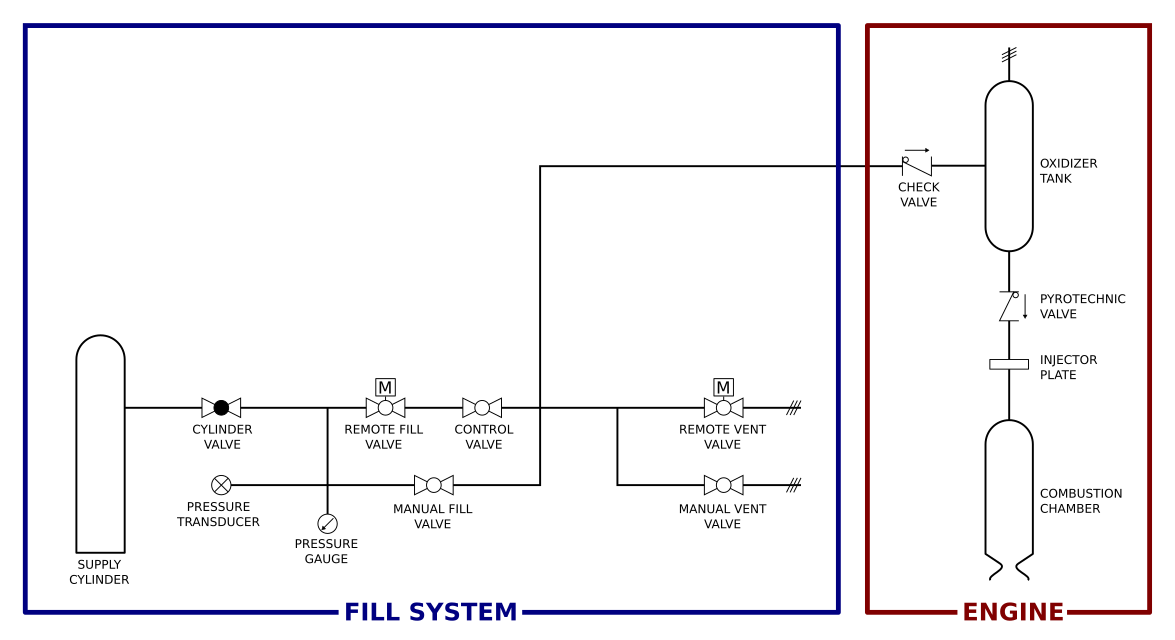
\includegraphics[width=0.75\textwidth]{images/PIDnoP}
\centering
\caption{P\&ID for the Vidar III engine and fill system}
\label{fig:launchPID}
\end{figure}
% end final setup checklist -- }}}


\end{document}
